\subsection{O5: real blurred license plates}
\label{sec:real}
\paragraph{Protocol.} Held-out subsets of two public datasets, disjoint from the development subsets:
\textbf{LPBlur}~\cite{lpblur2024} (400 pairs drawn; 397 whose sharp image yields a six-character
reading, which serves as the reference text) --- real motion blur of moving vehicles with paired
sharp exposures --- and \textbf{CCPD-Blur}~\cite{ccpd2018} (400 street photographs with annotated
plate text; the plate region plus a margin is restored). Restoration is RL with 30 iterations. OCR
reads the rectified plate; on 200 sharp CCPD plates it reads 99.8\% of the characters correctly,
so it is not the bottleneck. 95\% confidence intervals are bootstrap intervals over images.

\begin{table}[h]
\centering\small
\begin{tabular}{l|ccccc|cccc}
\toprule
 & \multicolumn{5}{c|}{LPBlur ($n=397$)} & \multicolumn{4}{c}{CCPD-Blur ($n=400$)} \\
system & char.\ acc. & exact & worse & PSNR & SSIM & char.\ acc. & exact & worse & accepted \\
\midrule
blurred input & 0.176 & 3.3\% & -- & 21.62 & 0.642 & \textbf{0.759} & \textbf{42.2\%} & -- & -- \\
classical baseline & 0.241 & 7.1\% & 19.1\% & 20.09 & 0.581 & 0.237 & 5.5\% & 84.5\% & 100\% \\
baseline + gate & 0.188 & 4.8\% & 1.8\% & 21.56 & 0.640 & 0.652 & 35.2\% & 21.5\% & 29\% \\
text-aware, no gate & \textbf{0.497} & 25.4\% & 9.8\% & 21.08 & 0.657 & 0.185 & 3.8\% & 87.5\% & 100\% \\
text-aware + gate & 0.407 & 19.9\% & \textbf{0.8\%} & \textbf{21.95} & \textbf{0.682} & 0.684 & 37.0\% & 14.0\% & 18\% \\
text-aware + strict gate & 0.308 & 13.6\% & 0.3\% & 21.85 & 0.666 & 0.726 & 40.2\% & 5.5\% & 7\% \\
text-aware, Wiener & \textbf{0.497} & \textbf{26.7\%} & 9.3\% & 21.37 & 0.658 & 0.215 & 5.2\% & 85.2\% & 100\% \\
\bottomrule
\end{tabular}
\caption{Held-out real plates. \emph{char.\ acc.}: OCR character accuracy (95\% CIs: LPBlur
blurred 0.149--0.203, text-aware 0.459--0.536, text-aware + gate 0.366--0.447; CCPD blurred
0.730--0.786, text-aware + gate 0.652--0.718). \emph{exact}: whole plate read correctly.
\emph{worse}: images whose OCR accuracy drops. LPBlur accepted rates: baseline + gate 10\%,
text-aware + gate 43\%, strict 24\%.}
\label{tab:real}
\end{table}

\begin{figure}[h]
\centering
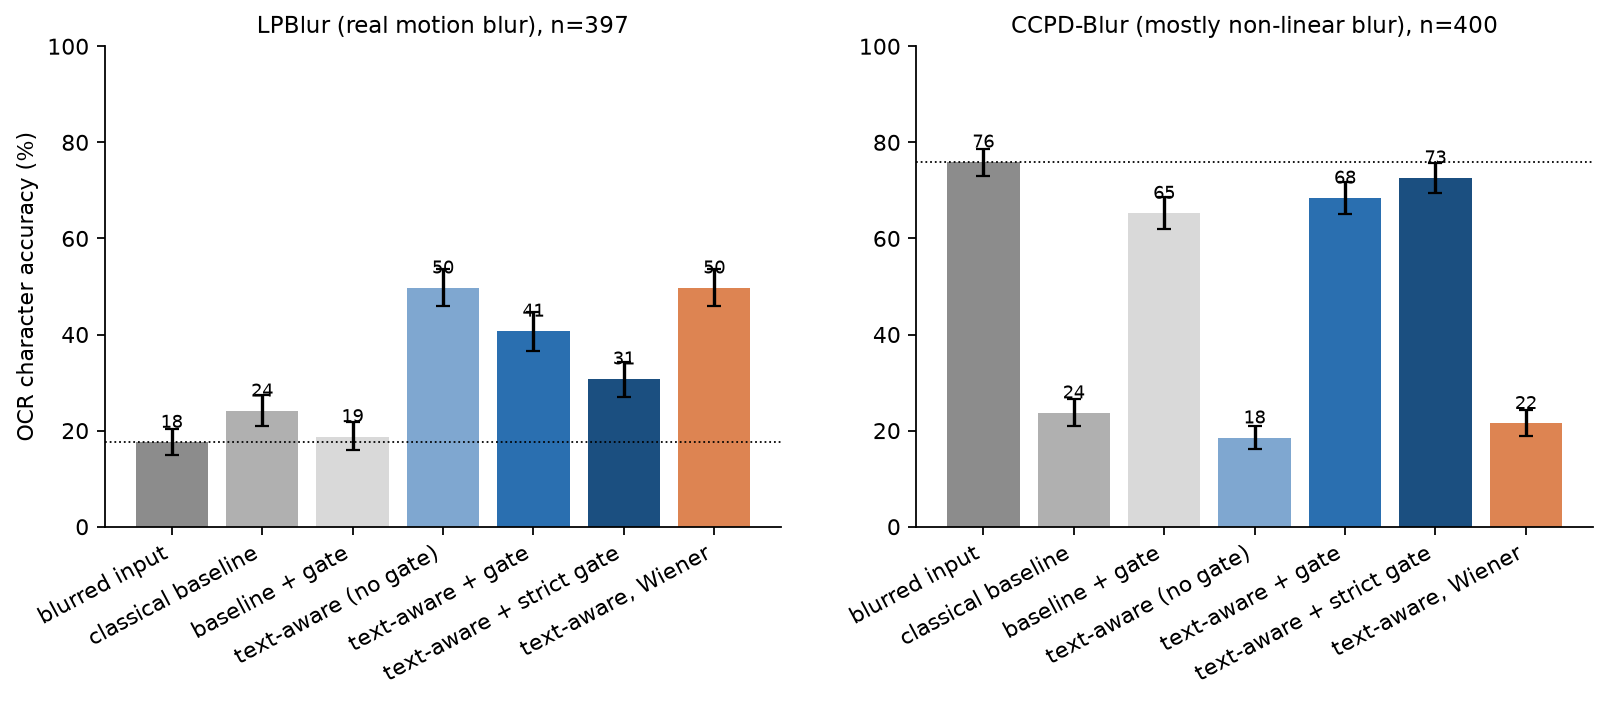
\includegraphics[width=\textwidth]{05_real_ocr.png}
\caption{OCR character accuracy on held-out real plates (dotted: blurred input).}
\label{fig:real}
\end{figure}

\paragraph{LPBlur: real motion blur.} The classical baseline lifts OCR accuracy only from 0.18 to
0.24 and makes 19\% of the plates worse; it also \emph{lowers} PSNR and SSIM. The text-aware estimator
reaches 0.50 --- almost three times the blurred input and twice the baseline --- and reads 25\% of
plates exactly, against 3\% blurred. The difference to the baseline lies entirely in the estimate
(both use the same RL), i.e.\ in the band limit (Section~\ref{sec:design}). With the gate, 43\% of the
plates are restored; only 0.8\% of all plates get worse, the mean accuracy is 0.41 (still $2.3\times$ the
input), and PSNR and SSIM are the best of all systems because no restoration with ringing gets
through. The gate withholds 96 restorations that would have helped, the price of refusing all but 3
of the 39 that would have hurt. Wiener with the same estimate performs on par with RL.

\paragraph{CCPD-Blur: mostly not linear motion.} Restoring every image with a line kernel is
destructive: accuracy falls from 0.76 to 0.19--0.24 and 85--88\% of the plates get worse --- the blur
in this set is predominantly defocus, mixed or non-uniform, which a straight line cannot explain,
and the plates are often already partly legible (42\% read exactly before restoration). The gate refuses 82\% of the images and recovers most of the loss
(0.68); the strict operating point refuses 93\% and comes within 3 points of the input (0.73). Neither
\emph{improves} on leaving CCPD-Blur alone, and we do not claim it does: the contribution of the
pipeline on this set is to recognise, for most images, that it should not act.

\begin{figure}[h]
\centering
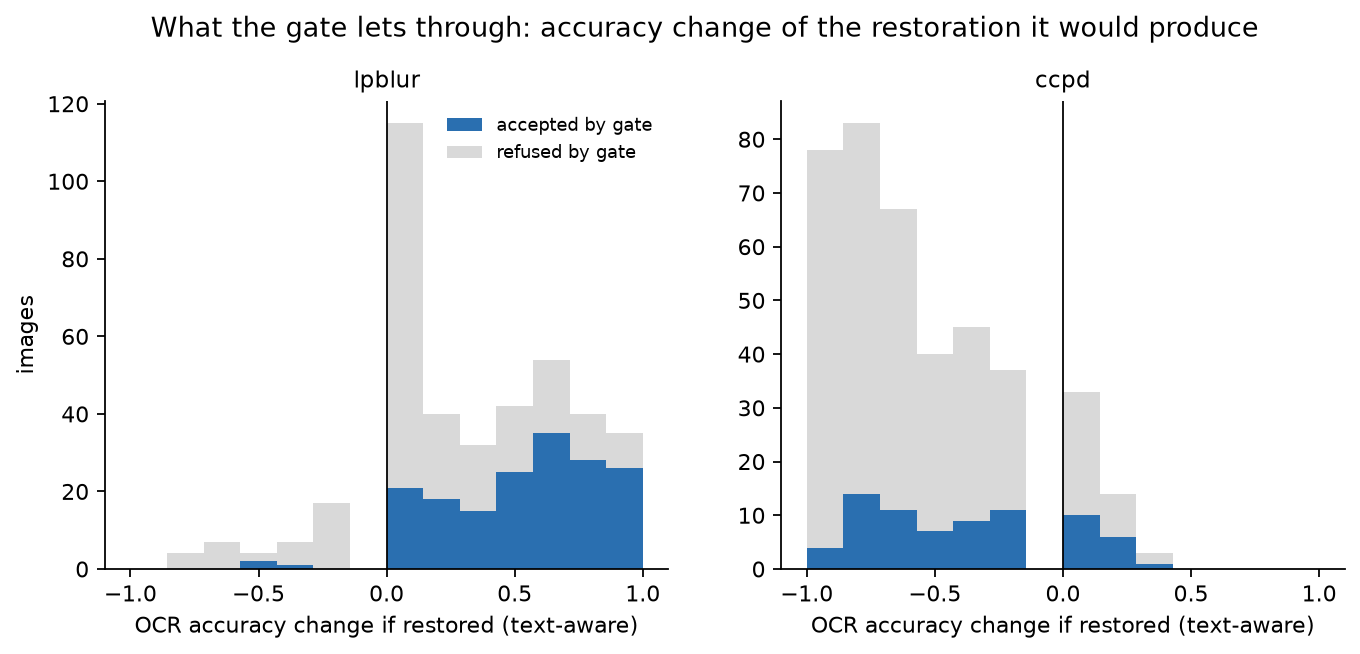
\includegraphics[width=0.9\textwidth]{05_gate_real.png}
\caption{Accuracy change the text-aware restoration would produce, split by the gate's decision.
On LPBlur the accepted cases are almost all improvements; on CCPD-Blur the gate refuses most
images, but a minority of the accepted ones still lose accuracy (the zero bin holds unchanged
readings).}
\label{fig:gatereal}
\end{figure}
